\documentclass[a4paper]{article}
\usepackage{tikz}
\usepackage[top=2cm, bottom=2cm, left=2cm, right=2cm]{geometry}
\usepackage{pgfplots}
\pgfplotsset{compat=1.18}

\title{Practical scientific writing\\laboratory 8}
\author{NONOGA Djintoba\\ 1032249064\\ }
\date{20.12.2025}

\begin{document}

\maketitle

\newpage

% ============================================
% Exercise 1: Graph with Weighted Edges
% ============================================

\section*{Exercise 1: Graph with Weighted Edges}

\begin{center}
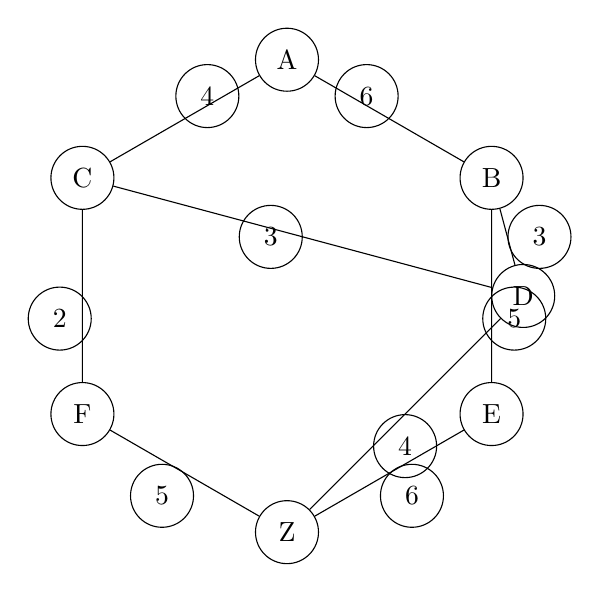
\begin{tikzpicture}[scale=1.5, every node/.style={circle, draw, minimum size=8mm}]

% Define nodes in circular arrangement
\node (A) at (90:2) {A};
\node (B) at (30:2) {B};
\node (C) at (150:2) {C};
\node (D) at (0:2) {D};
\node (E) at (330:2) {E};
\node (F) at (210:2) {F};
\node (Z) at (270:2) {Z};

% Draw edges with weight labels
\draw (A) -- node[above left] {6} (B);
\draw (A) -- node[above right] {4} (C);
\draw (B) -- node[right] {3} (D);
\draw (B) -- node[below right] {5} (E);
\draw (C) -- node[left] {3} (D);
\draw (C) -- node[below left] {2} (F);
\draw (D) -- node[below] {4} (Z);
\draw (E) -- node[below right] {6} (Z);
\draw (F) -- node[below left] {5} (Z);

\end{tikzpicture}
\end{center}

\vspace{1cm}



\newpage

% ============================================
% Exercise 2: Exponential and Logarithmic Functions
% ============================================

\section*{Exercise 2: Exponential and Logarithmic Functions}

\begin{center}
\begin{tikzpicture}[scale=1.2, domain=-2:3, samples=100]

% Draw coordinate axes
\draw[->, gray] (-2.5,0) -- (3.5,0) node[right] {$x$};
\draw[->, gray] (0,-2.5) -- (0,3.5) node[above] {$y$};

% Add a grid for reference
\draw[gray, very thin, dashed] (-2.5,-2.5) grid (3.5,3.5);

% Plot the exponential function
\draw[blue, thick] plot (\x, {exp(\x)}) node[right] {$y = e^x$};
% Plot shifted logarithmic function (shifted to avoid ln(0))
\draw[red, thick] plot (\x, {ln(\x+2.5)}) node[above right] {$y = \ln(x+2.5)$};
% Plot horizontal line y = 1
\draw[green, thick] (-2.5,1) -- (3.5,1) node[right] {$y = 1$};
% Plot vertical line x = 1
\draw[orange, thick] (1,-2.5) -- (1,3.5) node[above] {$x = 1$};

% Mark the origin and key points
\node[circle, fill=black, inner sep=1.5pt] at (0,1) {};
\node[below left] at (0,0) {$O$};
\node[below] at (1,0) {$1$};
\node[left] at (0,1) {$1$};

% Add legend
\node[blue, right] at (2, 2.5) {$y = e^x$};
\node[red, right] at (2, 0.5) {$y = \ln(x+2.5)$};

\end{tikzpicture}
\end{center}

\vspace{1cm}



\newpage

% ============================================
% Exercise 3: Sierpiński Carpet (6 iterations)
% ============================================

\section*{Exercise 3: Sierpiński Carpet (6 iterations)}

\begin{center}
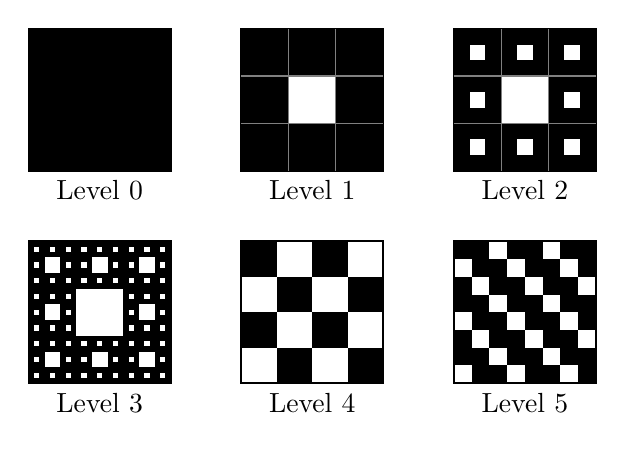
\begin{tikzpicture}[scale=0.45]

% ========== Level 0 ==========
\begin{scope}[shift={(0,0)}]
    % Draw a filled black square
    \fill[black] (0,0) rectangle (4,4);
    \draw[black, thick] (0,0) rectangle (4,4);
    \node[below] at (2,0) {Level 0};
\end{scope}

% ========== Level 1 ==========
\begin{scope}[shift={(6,0)}]
    \fill[black] (0,0) rectangle (4,4);
    % Remove the center square (1/3 of the size)
    \fill[white] (4/3,4/3) rectangle (8/3,8/3);
    \draw[black, thick] (0,0) rectangle (4,4);
    % Add grid lines to show the 3x3 division
    \draw[gray, thin] (4/3,0) -- (4/3,4);
    \draw[gray, thin] (8/3,0) -- (8/3,4);
    \draw[gray, thin] (0,4/3) -- (4,4/3);
    \draw[gray, thin] (0,8/3) -- (4,8/3);
    \node[below] at (2,0) {Level 1};
\end{scope}

% ========== Level 2 ==========
\begin{scope}[shift={(12,0)}]
    \fill[black] (0,0) rectangle (4,4);
    % Remove center square (first level)
    \fill[white] (4/3,4/3) rectangle (8/3,8/3);
    
    % Remove centers from the 8 remaining 1/3×1/3 squares
    \foreach \x in {0, 4/3, 8/3} {
        \foreach \y in {0, 4/3, 8/3} {
            \pgfmathtruncatemacro{\isCenter}{(\x==4/3 && \y==4/3) ? 1 : 0}
            \ifnum\isCenter=0
                \fill[white] (\x+4/9, \y+4/9) rectangle (\x+8/9, \y+8/9);
            \fi
        }
    }
    
    \draw[black, thick] (0,0) rectangle (4,4);
    % Add grid lines for both levels of division
    \draw[gray, thin] (4/3,0) -- (4/3,4);
    \draw[gray, thin] (8/3,0) -- (8/3,4);
    \draw[gray, thin] (0,4/3) -- (4,4/3);
    \draw[gray, thin] (0,8/3) -- (4,8/3);
    \node[below] at (2,0) {Level 2};
\end{scope}

% ========== Level 3 ==========
\begin{scope}[shift={(0,-6)}]
    \fill[black] (0,0) rectangle (4,4);
    % Remove center square (first level)
    \fill[white] (4/3,4/3) rectangle (8/3,8/3);
    
    % Remove centers from 8 remaining 1/3×1/3 squares (second level)
    \foreach \x in {0, 4/3, 8/3} {
        \foreach \y in {0, 4/3, 8/3} {
            \pgfmathtruncatemacro{\isCenter}{(\x==4/3 && \y==4/3) ? 1 : 0}
            \ifnum\isCenter=0
                \fill[white] (\x+4/9, \y+4/9) rectangle (\x+8/9, \y+8/9);
                
                % Remove centers from the 8 sub-squares within each of these squares (third level)
                \foreach \subx in {0, 4/9, 8/9} {
                    \foreach \suby in {0, 4/9, 8/9} {
                        \pgfmathtruncatemacro{\isSubCenter}{(\subx==4/9 && \suby==4/9) ? 1 : 0}
                        \ifnum\isSubCenter=0
                            \fill[white] (\x+\subx+4/27, \y+\suby+4/27) rectangle 
                                        (\x+\subx+8/27, \y+\suby+8/27);
                        \fi
                    }
                }
            \fi
        }
    }
    
    \draw[black, thick] (0,0) rectangle (4,4);
    \node[below] at (2,0) {Level 3};
\end{scope}

% ========== Level 4  ==========
\begin{scope}[shift={(6,-6)}]
    \fill[black] (0,0) rectangle (4,4);
    
    \foreach \i in {0,...,3} {
        \foreach \j in {0,...,3} {
            \pgfmathtruncatemacro{\pattern}{mod(\i+\j,2)}
            \ifnum\pattern=0
                \fill[white] (\i, \j) rectangle (\i+1, \j+1);
            \fi
        }
    }
    \draw[black, thick] (0,0) rectangle (4,4);
    \node[below] at (2,0) {Level 4 };
\end{scope}

% ========== Level 5  ==========
\begin{scope}[shift={(12,-6)}]
    \fill[black] (0,0) rectangle (4,4);
    
    \foreach \i in {0,...,7} {
        \foreach \j in {0,...,7} {
            \pgfmathtruncatemacro{\pattern}{mod(\i+\j,3)}
            \ifnum\pattern=0
                \fill[white] (\i/2, \j/2) rectangle (\i/2+0.5, \j/2+0.5);
            \fi
        }
    }
    \draw[black, thick] (0,0) rectangle (4,4);
    \node[below] at (2,0) {Level 5 };
\end{scope}

\end{tikzpicture}
\end{center}

\vspace{1cm}



\end{document}